% 开头模版
\documentclass[UTF8,fontset=macnew]{book} % 声明文档格式

% 导言区
% 包引用
\usepackage{ctex} % 中文支持包[模版内置]
\usepackage{titletoc} % 中文目录支持
\usepackage{amsmath}
\usepackage{amssymb}
\usepackage{color}
\usepackage{bm}
\usepackage{xcolor}
\usepackage{soul}
\usepackage{tikz}
\usetikzlibrary{calc,angles,quotes}
\usepackage{hyperref}
\usepackage{pifont}
\usepackage{tkz-euclide}




% 标题与作者
\title{课本命题及推导过程}
\author{唐凤廷}

% 命令支持
\renewcommand{\contentsname}{目录}
\newcommand{\mathcolorbox}[2]{\colorbox{#1}{$\displaystyle #2$}}
\newcommand{\feq}{\scalebox{-1}[1]{$\cong$}}
\definecolor{hlcolor}{RGB}{255,251,210}
\definecolor{hlblue}{RGB}{4,165,218}
\definecolor{hlred}{RGB}{216,18,126}
\hypersetup{
	colorlinks=true,
	linkcolor=black
}


% 文档正文

\begin{document}
\maketitle % 显示标题
{\fangsong
\begin{center}
	引言
\end{center}

在本书开头,我必须要说的是,人民教育出版社出版的《义务教育教科书 数学》系列教材是一套非常优秀的教材,也是本书的源头.

不过,该教材中含有许多的练习题和拓展知识,在学生复习时这些都可能成为干扰内容. 为便于学生复习,我使用\LaTeX 语言,对本书知识定理部分进行重排和重绘.

这是一项艰难的工作,课本上不仅有数十万字,更有许许多多的插图,我会将大部分插图进行矢量重绘,但部分图片我可能会略过. 这并不说明原书插图不会,而是重绘插图占用很多时间,我技术和精力有限,因此无法考虑所有的插图,希望各位读者理解.

我会尽我所能将本书做得与原教材相似,但因我能力有限,很多公式和插图很难与原教材达到同等水准,望各位读者理解.

为了实现本书的宗旨,本书的所有源代码将开源并定期更新. 为方便其他同学和读者再编译,编译本书使用的软件为Mac端的TeXstudio,采用\LaTeXe 编译.

最后,我申明,本书仅是原教材部分内容的搬运,不能代替原教材,同时本书仅用于教育用途,不以盈利为目的,故不构成侵权.
}
\tableofcontents % 显示目录

	% 请在下面输入文档正文
	\chapter{第一章\ 有理数}
		\section{正数和负数}
		
		\section{有理数}
			\subsection{有理数}
			
			\subsection{数轴}
			
			\subsection{相反数}
			
			\subsection{绝对值}
	
	\chapter{第二章\ 整式的加减}
	
	\chapter{第三章\ 一元一次方程}
	
	\chapter{第四章\ 几何图形初步}
	
	\chapter{第五章\ 相交线与平行线}
	
	\chapter{第六章\ 实数}
	
	\chapter{第七章\ 平面直角坐标系}
	
	\chapter{第八章\ 二元一次方程}
	
	\chapter{第九章\ 不等式与不等式组}
	
	\chapter{第十章\ 数据的收集、整理与描述}
	
	\chapter{第十一章\ 三角形}
		\section{与三角形有关的线段}
			\subsection{三角形的边}
				由不在同一条直线上的三条线段收尾顺次相接组成的图形叫做\textcolor[RGB]{4,165,218}{\bm{{\heiti 三角形}}} (triangle).
				
				在图$11.\ 1$-$1$中,线段$AB$,$BC$,$CA$是三角形的边. 点$A,\ B,\ C$是三角形的顶点. $\angle A,\ \angle B,\ \angle C$是相邻两边组成的角,叫做三角形的内角,简称三角形的角.
				
				顶点是$A,\ B,\ C$的三角形,记作$\triangle ABC$,读作“三角形$ABC$”.
				
				$\triangle ABC$的三边,有时用$a,\ b,\ c$来表示. 如图$11.\ 1$-$1$,顶点$A$所对的边$BC$用$a$表示,顶点$B$所对的边$AC$用$b$表示,顶点$C$所对的边$AB$用$c$表示.
				\begin{center}
					\begin{tikzpicture}
						\coordinate (B) at (0,0);
						\coordinate (A) at (3,3);
						\coordinate (C) at (5,0);
						
						\draw (A) - - (B);
						\draw (B) - - (C);
						\draw (C) - - (A);
						
						\node at (A) [above] {$A$};
						\node at (B) [left] {$B$};
						\node at (C) [right] {$C$};
						
						\draw pic[draw, hlblue] {angle=C--B--A};
						\draw pic[draw, hlblue] {angle=B--A--C};
						\draw pic[draw, hlblue] {angle=A--C--B};
						
						\node at (2.56,-0.44) {$a$};
						\node at (4.17,1.66) {$b$};
						\node at  (1.36,1.70) {$c$};
					\end{tikzpicture}
					\\图$11.\ 1$-$1$
				\end{center}
				
				我们知道:三边相等的三角形叫做等边三角形(图$11.\ 1$-$2\ (1)\ $);有两条边相等的三角形叫做等腰三角形(图$11.\ 1$-$2\ (2)\ $).
				
				图$11.\ 1$-$2\ (3)\ $中的三角形是三边都不相等的三角形.
				\begin{center}
					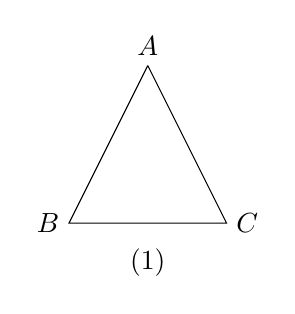
\begin{tikzpicture}
						\coordinate (A) at (1,2);
						\coordinate (B) at (0,0);
						\coordinate (C) at (2,0);
						
						\draw (A) - - (B) - - (C) - - (A);
						
						\node at (A) [above] {$A$};
						\node at (B) [left] {$B$};
						\node at (C) [right] {$C$};
						\node at (1,-0.5) {$(1)$};
					\end{tikzpicture}
					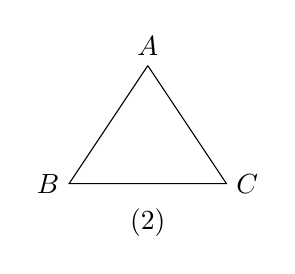
\begin{tikzpicture}
						\coordinate (A) at (1,1.5);
						\coordinate (B) at (0,0);
						\coordinate (C) at (2,0);
						
						\draw (A) - - (B) - - (C) - - (A);
						
						\node at (A) [above] {$A$};
						\node at (B) [left] {$B$};
						\node at (C) [right] {$C$};
						\node at (1,-0.5) {$(2)$};
					\end{tikzpicture}
					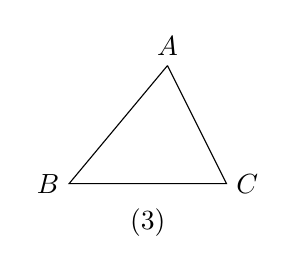
\begin{tikzpicture}
						\coordinate (A) at (1.25,1.5);
						\coordinate (B) at (0,0);
						\coordinate (C) at (2,0);
						
						\draw (A) - - (B) - - (C) - - (A);
						
						\node at (A) [above] {$A$};
						\node at (B) [left] {$B$};
						\node at (C) [right] {$C$};
						\node at (1,-0.5) {$(3)$};
					\end{tikzpicture}
					\\ 图$11.\ 1$-$2$
				\end{center}
				
				以“是否有边相等“,可以将三角形分为两类:三边都不相等的三角形和等腰三角形.
				
				我们还知道:在等腰三角形中,相等的两边都叫做腰,另一边叫做底边,两腰的夹角叫做顶角,腰和底边的夹角叫做底角.
				
				等边三角形是特殊的等腰三角形,即底边和腰相等的等腰三角形.
				
				综上,三角形按边的相等关系分类如下:
				
				$\text{三角形} \begin{cases}\text{三边都不相等的三角形}\\\text{等腰三角形}\begin{cases}\text{腰和底边不相等的等腰三角形} \\\text{等边三角形} \end{cases}  \end{cases}$
				
				下面探究三角形三边之间的大小关系.
				
				对于任意一个·$\triangle ABC$,如果把其中任意两个顶点(例如$B,\ C$)看成顶点,由“两点之间,线段最短”可得
			\begin{align}AB+AC>BC.\tag{1} \end{align}
			同理有
			\begin{align}AC+BC>AB\tag{2},\\AB+BC>AC\tag{3} .\end{align}
				
				一般,我们有
				
				\textcolor[RGB]{4,165,218}{\bm{{\heiti 三角形两边的和大于第三边.}}}
				
				由不等式(2)(3)移项可得$BC>AB-AC,\ BC>AC-AB.$ 这就是说,\textcolor[RGB]{4,165,218}{\bm{{\heiti 三角形两边的差小于第三边.}}}
				\subsection{三角形的高、中线与角平分线}
					与三角形有关的线段,除了三条边,还有我们已经学过的三角形的高. 如图$11.\ 1$-$3$,从$\triangle ABC$的顶点$A$向它所对的边$BC$所在的直线画垂线,垂足为$D$,所得线段$AD$叫做$\triangle ABC$的边$BC$上的\textcolor[RGB]{4,165,218}{\bm{{\heiti 高}}} (altitude).
					
					\begin{center}
						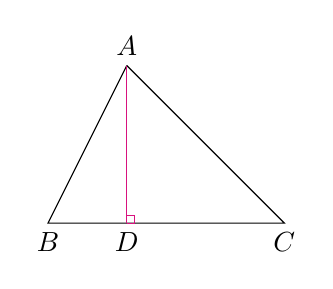
\begin{tikzpicture}
							\coordinate (A) at (1,2);
							\coordinate (B) at (0,0);
							\coordinate (C) at (3,0);
							\coordinate (D) at (1,0);
							
							\draw (A) - - (B) - - (C) - - (A);
							\draw[hlred] (A) - - (D);
							
							\tkzMarkRightAngle[size=.1, color=hlred](A,D,C);
							
							\node at (A) [above] {$A$};
							\node at (B) [below] {$B$};
							\node at (C) [below] {$C$};
							\node at (D) [below] {$D$};
						\end{tikzpicture}
						\\
						图$11.\ 1$-$3$
					\end{center}
					
					我们再来看两种与三角形有关的线段.
					
					如图$11.\ 1$-$4\ (1)$,连接$\triangle ABC$的顶点$A$和它所对的边$BC$的中点$D$,所得线段$AD$叫做$\triangle ABC$的边$BC$上的\textcolor[RGB]{4,165,218}{\bm{{\heiti 中线}}} (median).
					
					\begin{center}
						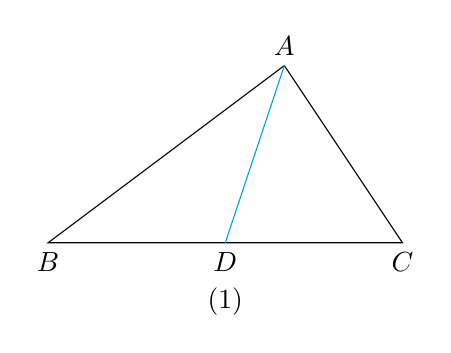
\begin{tikzpicture}
							\coordinate (A) at (3,2.25);
							\coordinate (B) at (0,0);
							\coordinate (C) at (4.5,0);
							\coordinate (D) at (2.25,0);
							
							\draw (A) - - (B) - - (C) - - (A);
							\draw[hlblue] (A) - - (D);
							
							\node at (A) [above] {$A$};
							\node at (B)[below] {$B$};
							\node at (C) [below] {$C$};
							\node at (D) [below] {$D$};
							
							\node at (2.25,-0.75) {$(1)$};
						\end{tikzpicture}
						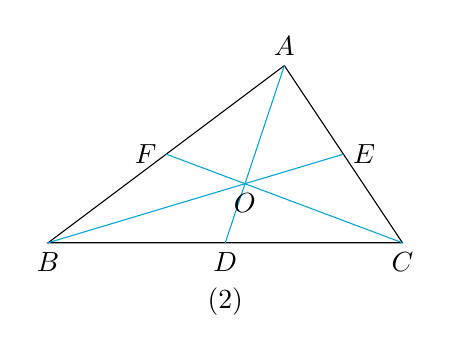
\begin{tikzpicture}
							\coordinate (A) at (3,2.25);
							\coordinate (B) at (0,0);
							\coordinate (C) at (4.5,0);
							\coordinate (D) at (2.25,0);
							\tkzDefMidPoint(A,B) \tkzGetPoint{F};
							\tkzDefMidPoint(A,C) \tkzGetPoint{E};
							\tkzDefTriangleCenter[centroid](A,B,C) \tkzGetPoint{O}

							\draw (A) - - (B) - - (C) - - (A);
							\draw[hlblue] (A) - - (D);
							\draw[hlblue] (B) - - (E);
							\draw[hlblue] (C) - - (F);

							\node at (A) [above] {$A$};
							\node at (B)[below] {$B$};
							\node at (C) [below] {$C$};
							\node at (D) [below] {$D$};
							\node at (E) [right] {$E$};
							\node at (F) [left] {$F$};
							\node at (O) [below] {$O$};

							\node at (2.25,-0.75) {$(2)$};
							

						\end{tikzpicture}
						\\
						图$11.\ 1$-$4$
					\end{center}
					
					如图$11.\ 1$-$4\ (2)$,三角形的三条中线相交与一点. 三角形三条中线的交点叫做\textcolor[RGB]{4,165,218}{\bm{{\heiti 三角形的重心}}}.
					
					\begin{center}
						\begin{tikzpicture}
							\coordinate (A) at (2,3);
							\coordinate (B) at (0,0);
							\coordinate (C) at (6,0);
							\coordinate (D) at (2.51,0);
							
							\draw (A)- - (B) - - (C) - - (A);
							\draw[hlred] (A) - - (D);
							
							\draw pic[draw, hlblue] {angle=B--A--D};
							\draw pic[draw, hlblue, angle radius=0.6cm] {angle=D--A--C};
							
							\node at (A) [above] {$A$};
							\node at (B) [below] {$B$};
							\node at (C) [below] {$C$};
							\node at (D) [below] {$D$};
						\end{tikzpicture}
						\\
						图$11.\ 1$-$5$
					\end{center}
					
					如图$11.\ 1$-$5$,画$\angle A$的平分线$AD$,交$\angle A$所对的边$BC$于点$D$,所得线段$AD$叫做$\triangle ABC$的\textcolor[RGB]{4,165,218}{\bm{{\heiti 角平分线}}} (angular bisector).
				\subsection{三角形的稳定性}
				三角形是具有稳定性的图形,而四边形没有稳定性.
		\section{与三角形有关的角}
			\subsection{三角形的内角}
				\begin{center}
					\begin{tikzpicture}
						\coordinate (A) at (1.5,2);
						\coordinate (B) at (0,0);
						\coordinate (C) at (2.5,0);
						\coordinate (D) at (0,2);
						\coordinate (E) at (3,2);
						
						\draw (A) - - (B) - - (C) - - (A);
						\draw[hlblue, dashed] (D) - - (E);
						
						\draw pic["$1$", draw, black, angle eccentricity=1.5, angle radius=0.3cm] {angle=B--A--C};
						\draw pic["$2$", draw=hlblue!, angle eccentricity=1.5, angle radius=0.3cm] {angle=C--B--A};
						\draw pic["$3$", draw=hlred!, angle eccentricity=1.5, angle radius=0.3cm] {angle=A--C--B};
						\draw pic["$4$", draw=hlblue!, angle eccentricity=1.5, angle radius=0.3cm] {angle=D--A--B};
						\draw pic["$5$", draw=hlred!, angle eccentricity=1.5, angle radius=0.3cm] {angle=C--A--E};
						
						\node at (A) [above] {$A$};
						\node at (B) [left] {$B$};
						\node at (C) [right] {$C$};
						\node at (E) [above] {$l$};
						
						\node at (1.5,-0.5) {图$11.\ 2$-$2$};
					\end{tikzpicture}
				\end{center}
			
				已知:$\triangle ABC$(图$11.\ 2$-$2$).
			
				求证:$\angle A + \angle B + \angle C = 180^{\circ}.$
			
				\textcolor[RGB]{4,165,218}{\bm{{\heiti 证明:}}}如图$11.\ 2$-$2$,过点$A$作直线$l$,使$l//BC.$
			
				$\because \ l//BC,$
			
				$\therefore \ \angle 2 = \angle 4 \ (\text{两直线平行,内错角相等}).$
			
				同理   $\angle 3 = \angle 5.$
			
				$\because \ \angle 1,\ \angle 4,\ \angle 5$组成平角,
			
				$\therefore \  \angle 1 + \angle 4 +\angle 5 = 180^{\circ}\ (\text{平角定义}).$
			
				$\therefore \ \angle 1 + \angle 2 + \angle 3 = 180^{\circ}\ (\text{等量代换}).$
				
				以上我们就证明了任意一个三角形的内角和都等于$180^{\circ}$,得到如下定理:
				
				\bm{{\heiti 三角形内角和定理}}\ \ \ 	\textcolor[RGB]{4,165,218}{\bm{{\heiti 三角形三个内角的和等于}}$180^{\circ}$\bm{{\heiti .}}}
				
				\begin{center}
					\begin{tikzpicture}
						\coordinate (A) at (2,4);
						\coordinate (B) at (0,0);
						\coordinate (C) at (2,0);
						
						\draw (A) - - (B) - - (C) - - (A);
						
						\tkzMarkRightAngle[size=.15, color=hlred](B,C,A);
						
						\node at (A) [above] {$A$};
						\node at (B) [left] {$B$};
						\node at (C) [right] {$C$};
						
						\node at (1,-0.5) {图$11.\ 2$-$5$};
					\end{tikzpicture}
				\end{center}
				
				如图$11.\ 2$-$5$,在直角三角形$ABC$中,$\angle C = 90^{\circ} $,由三角形内角和定理,得
			$$\angle A + \angle B + \angle C =180^{\circ},$$
			即
			$$\angle A + \angle B + 90^{\circ} =180^{\circ},$$
			所以
			$$\angle A + \angle B = 90^{\circ}.$$
			
				也就是说,\textcolor[RGB]{4,165,218}{\bm{{\heiti 直角三角形的两个锐角互余.}}}
				
				直角三角形可以用符号\ “Rt$\triangle$”\ 表示,直角三角形$ABC$可以写成$\text{Rt}\triangle ABC.$
				
				由三角形内角和定理可得:
				
				\textcolor[RGB]{4,165,218}{\bm{{\heiti 有两个角互余的三角形是直角三角形.}}}
			\subsection{三角形的外角}
				\begin{center}
					\begin{tikzpicture}
						\coordinate (A) at (3,3);
						\coordinate (B) at (0,0);
						\coordinate (C) at (4,0);
						\coordinate (D) at (5,0);
						
						\draw (A) - - (B) - - (C) - - (A);
						\draw (C) - - (D);
						
						\draw pic[draw=hlblue!, angle radius=0.3cm] {angle=D--C--A};
						
						\node at (A) [above] {$A$};
						\node at (B) [below] {$B$};
						\node at (C) [below] {$C$};
						\node at (D) [below] {$D$};
						\node at (2.5,-0.75) {图$11.\ 2$-$7$};
					\end{tikzpicture}
				\end{center}
				
				如图$11.\ 2$-$7$,把$\triangle ABC$的一边$BC$延长,得到$\angle ACD$. 像这样,三角形的一边与另一边的延长线组成的角,叫做\textcolor[RGB]{4,165,218}{\bm{{\heiti 三角形的外角}}}.
				
				一般地,由三角形内角和定理可以推出下面的推论(请同学们自己证明):
				
				\textcolor[RGB]{4,165,218}{\bm{{\heiti 三角形的外角等于与它不相邻的两个内角的和.}}}
		\section{多边形及其内角和}
			\subsection{多边形}
			我们学过三角形. 类似地,在平面内,由一些线段收尾顺次相接组成的封闭图形叫做\textcolor[RGB]{4,165,218}{\bm{{\heiti 多边形}}} (polygon).
			
			多边形相邻两边组成的角叫做它的内角. 图$11.\ 3$-$3$中的$\angle A$,$\angle B$,$\angle C$,$\angle D$,$\angle E$是五边形$ABCDE$的$5$个内角. 多边形的边与它的邻边的延长线组成的角叫做多边形的外角. 图$11.\ 3$-$4$中的$\angle 1$是五边形$ABCDE$的一个外角.
			
			\begin{center}
				\begin{tikzpicture}
					\coordinate (A) at (1.5,2.5);
					\coordinate (B) at (0,1.5);
					\coordinate (C) at (0,0);
					\coordinate (D) at (2.5,0);
					\coordinate (E) at (3,1);
					
					\draw (A) - - (B) - - (C) - - (D) - - (E) - - (A);
					
					\node at (A) [above] {$A$};
					\node at (B) [left] {$B$};
					\node at (C) [left] {$C$};
					\node at (D) [right] {$D$};
					\node at (E) [right] {$E$};
					\node at (1.5,-0.75) {图$11.\ 3$-$3$};
				\end{tikzpicture}
				\begin{tikzpicture}
					\coordinate (A) at (1.5,2.5);
					\coordinate (B) at (0,1.5);
					\coordinate (C) at (0,0);
					\coordinate (D) at (2.5,0);
					\coordinate (E) at (3,1);
					\coordinate (F) at (2,2.83);
					
					\draw (A) - - (B) - - (C) - - (D) - - (E) - - (A);
					\draw (A) - - (F);
					\draw pic["$1$", draw=hlblue!, angle eccentricity=1.5, angle radius=0.3cm] {angle=E--A--F};
					
					\node at (A) [above] {$A$};
					\node at (B) [left] {$B$};
					\node at (C) [left] {$C$};
					\node at (D) [right] {$D$};
					\node at (E) [right] {$E$};
					\node at (1.5,-0.75) {图$11.\ 3$-$4$};
				\end{tikzpicture}
			\end{center}
			
			连接多边形不相邻的两个顶点的线段,叫做多边形的\textcolor[RGB]{4,165,218}{\bm{{\heiti 对角线}}} (diagonal). 图$11.\ 3$-$5$中,$AC$,$AD$是五边形$ABCDE$的两条对角线.
			
			\begin{center}
				\begin{tikzpicture}
					\coordinate (A) at (1.5,2.5);
					\coordinate (B) at (0,1.5);
					\coordinate (C) at (0.5,0);
					\coordinate (D) at (2,0);
					\coordinate (E) at (2.5,1.75);
					
					\draw (A) - - (B) - - (C) - - (D) - - (E) - - (A);
					\draw[hlblue] (A) - - (C);
					\draw[hlblue] (A) - -(D);
					
					\node at (A) [above] {$A$};
					\node at (B) [left] {$B$};
					\node at (C) [below] {$C$};
					\node at (D) [below] {$D$};
					\node at (E) [right] {$E$};
					\node at (1.25,-0.75) {图$11.\ 3$-$5$};
				\end{tikzpicture}
			\end{center}
							
							如图$11.\ 3$-$6\ (1)$,画出四边形$ABCD$的任何一条边(例如$CD$)所在直线,整个四边形都在这条直线的同一侧,这样的四边形叫做凸四边形. 而图$11.\ 3$-$6\ (2)$中的四边形$ABCD$就不是凸四边形,因为画出边$CD$(或$BC$)所在直线,整个四边形不都在这条直线的同一侧. 类似地,画出多边形的任何一条边所在直线,如果整个多边形都在这条直线的同一侧,那么这个多边形就是凸多边形. 本节只讨论凸四边形.
			
			\begin{center}
				\begin{tikzpicture}
					\coordinate (A) at (2,2.5);
					\coordinate (B) at (0.75,1.5);
					\coordinate (C) at (1.5,0);
					\coordinate (D) at (3,0);
					\coordinate (E) at (0,0);
					\coordinate (F) at (3.5,0);
					
					\draw (A) - - (B) - - (C) - - (D) - - (A);
					\draw[hlred, dashed] (E) - - (C);
					\draw[hlred, dashed] (D) - -(F);
					
					\node at (A) [above] {$A$};
					\node at (B) [left] {$B$};
					\node at (C) [below] {$C$};
					\node at (D) [below] {$D$};
					\node at (1.75,-0.75) {$(1)$};
				\end{tikzpicture}
				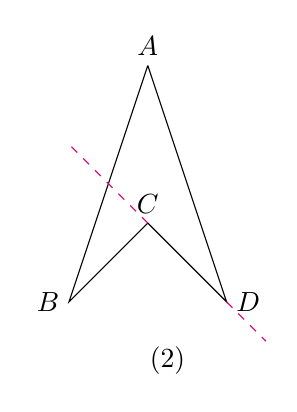
\begin{tikzpicture}
					\coordinate (A) at (1,3);
					\coordinate (B) at (0,0);
					\coordinate (C) at (1,1);
					\coordinate (D) at (2,0);
					\coordinate (E) at (0,2);
					\coordinate (F) at (2.5,-0.5);
					
					\draw (A) - - (B) - - (C) - - (D) - - (A);
					\draw[hlred, dashed] (C) - - (E);
					\draw[hlred, dashed] (D) - - (F);
					
					\node at (A) [above] {$A$};
					\node at (B) [left] {$B$};
					\node at (C) [above] {$C$};
					\node at (D) [right] {$D$};
					\node at (1.25,-0.75) {$(2)$};
				\end{tikzpicture}
				\\
				图$11.\ 3$-$6$
			\end{center}
			
			我们知道,正方形的各个角都相等,各条边都相等. 像正方形这样,各个角都相等,各条边都相等的多边形叫做\textcolor[RGB]{4,165,218}{\bm{{\heiti 正多边形}}} (regular polygon). 图$11.\ 3$-$7$是正多边形的一些例子.
			
			\begin{center}
				\begin{tikzpicture}
					\draw[hlred] (0,0) - - (1,1.73) - - (2,0) - - (0,0);
					\node at (1,-0.5) {正三角形};
				\end{tikzpicture}
				\begin{tikzpicture}
					\draw[hlred] (0,0) - - (0,2) - - (2,2) - - (2,0) - - (0,0);
					\node at (1,-0.5) {正方形};
				\end{tikzpicture}
				\begin{tikzpicture}
					\draw[hlred] (0,0) - - (2,0) - - (2.62,1.9) - - (1,3.08) - - (-0.62,1.9) - - (0,0);
					\node at (1,-0.5) {正五边形};
				\end{tikzpicture}
				\begin{tikzpicture}
					\draw[hlred] (0,0) - - (2,0) - - (3,1.73) - - (2,3.46) - - (0,3.46) - - (-1,1.73) - - (0,0);
					\node at (1,-0.5) {正六边形};
				\end{tikzpicture}
				\\
				图$11.\ 3$-$7$
			\end{center}
			\subsubsection{多边形的内角和}
				要用三角形内角和定理证明四边形的内角和等于$360^{\circ}$,只要将四边形分成几个三角形即可.
				
				\begin{center}
					\begin{tikzpicture}
						\coordinate (A) at (0,0);
						\coordinate (B) at (14/3,0);
						\coordinate (C) at (4,4/3);
						\coordinate (D) at (4/3,8/3);
						
						\draw (A) - - (B) - - (C) - - (D) - - (A);
						\draw[hlblue, dashed] (A) - - (C);
						\draw pic["$1$", draw=hlblue!, angle eccentricity=1.9, angle radius=0.5cm] {angle=B--A--C};
						\draw pic["$2$", draw=hlblue!, angle eccentricity=1.6, angle radius=0.3cm] {angle=C--A--D};
						\draw pic["$3$", draw=hlblue!, angle eccentricity=1.5, angle radius=0.3cm] {angle=A--C--B};
						\draw pic["$4$", draw=hlblue!, angle eccentricity=1.5, angle radius=0.5cm] {angle=D--C--A};
						
						\node at (A) [left] {$A$};
						\node at (B) [right] {$B$};
						\node at (C) [right] {$C$};
						\node at (D) [above] {$D$};
						\node at (7/3,-0.75) {图$11.\ 3$-$8$};
					\end{tikzpicture}
				\end{center}
				
				如图$11.\ 3$-$8$,在四边形$ABCD$中,连接对角线$AC$,则四边形$ABCD$被分为$\triangle ABC$和$\triangle ACD$两个三角形.
				
				由此可得
				
				$\begin{aligned}&\angle DAB+\angle B+\angle BCD+\angle D\\=&\angle 1+\angle 2+\angle B+\angle 3+\angle 4+\angle D\\=&(\angle 1+\angle B+\angle 3)+(\angle 2+\angle 4+\angle D).\end{aligned}$
				
				$\begin{aligned}\because \ &\angle 1+\angle B+\angle 3=180^{\circ},\\&\angle 2+\angle 4+\angle D=180^{\circ},\\\therefore \ &\angle DAB+\angle B+\angle BCD+\angle D=180^{\circ}+180^{\circ}=360^{\circ}.\end{aligned}$
			
				\noindent 即四边形的内角和等于$360^{\circ}.$
				
				一般地,从$n$边形的一个顶点出发,可以作$(n-3)$条对角线,它们将$n$边形分为$(n-2)$个三角形,$n$边形的内角和等于$180^{\circ} \times (n-2).$
				
				这样就得出了多边形内角和的公式:
				
				\textcolor[RGB]{4,165,218}{$n$\bm{{\heiti 边形内角和等于}}$(n-2)\times 180^{\circ}$\bm{{\heiti .}}}
				
				$n$边形的任何一个外角加上与它相邻的内角都等于$180^{\circ}$. 因此$n$边形的$n$个外角加上与他们相邻的内角,所得总和等于$n\times 180^{\circ}.$
				
				这个总和就是$n$边形的外角和加上内角和. 所以外角和等于总和减去内角和,即外角和等于
				$$n\times 180^{\circ} - (n-2)\times 180^{\circ}=2\times 180^{\circ}=360^{\circ}.$$
				
				由上面的思考可以得到:
				
				\textcolor[RGB]{4,165,218}{\bm{{\heiti 多边形的外角和等于}}$360^{\circ}$\bm{{\heiti .}}}
				
				你也可以像下面这样理解为什么多边形的外角和等于$360^{\circ}$.
				
				\begin{center}
					\begin{tikzpicture}
						\coordinate (A) at (0,0);
						\coordinate (A') at (0,-1);
						\coordinate (B) at (3,0);
						\coordinate (B') at (4,0);
						\coordinate (C) at (5,3);
						\coordinate (C') at (5.55,3.83);
						\coordinate (D) at (2,5);
						\coordinate (D') at (1.17,5.55);
						\coordinate (E) at (0,3);
						\coordinate (E') at (-0.71,2.29);
						
						\draw (A) - - (B) - - (C) - - (D) - - (E) - - (A);
						\draw (A) - - (A');
						\draw (B) - - (B');
						\draw (C) - - (C');
						\draw (D) - - (D');
						\draw (E) - - (E');
						
						\draw pic[->, draw=hlblue!, angle radius=0.3cm] {angle=A'--A--B};
						\draw pic[->, draw=hlblue!, angle radius=0.3cm] {angle=B'--B--C};
						\draw pic[->, draw=hlblue!, angle radius=0.3cm] {angle=C'--C--D};
						\draw pic[->, draw=hlblue!, angle radius=0.3cm] {angle=D'--D--E};
						\draw pic[->, draw=hlblue!, angle radius=0.3cm] {angle=E'--E--A};
						
						\coordinate (A") at (0.25,0.43);
						\coordinate (B") at (2.75,0.43);
						\coordinate (C") at (4.5,3.06);
						\coordinate (D") at (2.25,4.57);
						\coordinate (E") at (0.25,2.57);
						
						\draw [hlred, dashed] (A") - - (B") - - (C") - - (D") - - (E") - - (A");
						
						\node at (A) [left] {$A$};
						\node at (2.5,-1.75) {图$11.\ 3$-$12$};
					\end{tikzpicture}
				\end{center}
				
				如图$11.\ 3$-$12$,从多边形的一个顶点$A$出发,沿多边形的各边走过各顶点,再回到$A$,然后转向出发时的方向. 在行程中所转的各个角的和,就是多边形的外角和. 由于走了一周,所转的各个角的和等于一个周角,所以多边形的外角和等于$360^{\circ}.$
	\chapter{第十二章\ 全等三角形}
		\section{全等三角形}
			能够完全重合的两个图形叫做\textcolor[RGB]{4,165,218}{\bm{{\heiti 全等形}}} (congruent figures).
			
			能够完全重合的两个三角形叫做\textcolor[RGB]{4,165,218}{\bm{{\heiti 全等三角形}}} (congruent triangles).
			
			一个图形经过平移、翻折、旋转后,位置变化了,但形状、大小都没有改变,即平移、翻折、旋转前后的图形全等.
			
			把两个全等的三角形重合到一起,重合的顶点叫做\textcolor[RGB]{4,165,218}{\bm{{\heiti 对应顶点}}},重合的边叫做\textcolor[RGB]{4,165,218}{\bm{{\heiti 对应边}}},重合的角叫做\textcolor[RGB]{4,165,218}{\bm{{\heiti 对应角}}}.
			
			全等三角形有这样的性质:
			
			\textcolor[RGB]{4,165,218}{\bm{{\heiti 全等三角形的对应边相等,全等三角形的对应角相等.}}}
		\section{全等三角形的判定}
			\begin{center}
				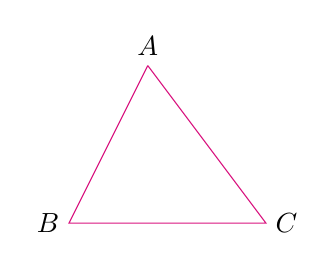
\begin{tikzpicture}
					\coordinate (A) at (1,2);
					\coordinate (B) at (0,0);
					\coordinate (C) at (2.5,0);
					
					\draw[hlred] (A) - - (B) - - (C) - - (A);
					
					\node at (A) [above] {$A$};
					\node at (B) [left] {$B$};
					\node at (C) [right] {$C$};
				\end{tikzpicture}
				\begin{tikzpicture}
					\coordinate (A) at (1,2);
					\coordinate (B) at (0,0);
					\coordinate (C) at (2.5,0);
					
					\draw[hlblue] (A) - - (B) - - (C) - - (A);
					
					\node at (A) [above] {$A'$};
					\node at (B) [left] {$B'$};
					\node at (C) [right] {$C'$};
				\end{tikzpicture}
				\\
				图$12.\ 2$-$1$
			\end{center}
			
			我们知道,如果$\triangle ABC\feq \triangle A'B'C'$\footnote{课本原文的全等符号无法在\LaTeX 语言中找到,故将\LaTeX 中错误的全等符号$\cong$水平翻转,得到正确的全等符号$\feq$. 下同.},那么它们的对应边相等,对应角相等. 反过来,根据全等三角形的定义,如果$\triangle ABC$与$\triangle A'B'C'$满足三条边分别相等,三个角分别相等,即
			$$\begin{gathered}
				AB=A'B',\ BC=B'C',\ CA=C'A',\\ \angle A=\angle A',\ \angle B=\angle B',\ \angle C=\angle C',
			\end{gathered}$$
			就能判定$\triangle ABC \feq \triangle A'B'C'\ (\text{图$12.\ 2$-$1$}).$
			
			一定要满足三条边分别相等,三个角也分别相等,才能保证两个三角形全等吗? 上述六个条件中,有些条件是相关的. 能否在上述六个条件中选择部分条件,简洁地判定两个三角形全等呢?
			
			本节我们就来讨论这个问题\footnote{本节证明过程繁多,为求简洁,故将探究部分删去,只保留结论,如有需要可自行查阅课本.}.
			
			通过画图可以发现,满足上述六个条件中的一个或两个,$\triangle ABC$与$\triangle A'B'C'$不一定全等. 满足上述六个条件中的三个,就能保证$\triangle ABC$与$\triangle A'B'C'$全等吗?
			
			我们分情况进行讨论.
			
			由探究$2$可以得到以下基本事实,用它可以判定两个三角形全等:
			
			\textcolor[RGB]{4,165,218}{\bm{{\heiti 三边分别相等的三角形全等}}}\ (可以简写成\ “边边边”\ 或\ “SSS”\ ).
		\section{角的平分线的性质}
		
	\chapter{第十三章\ 轴对称}
		\section{轴对称}
			\subsection{轴对称}
			
			\subsection{线断的垂直平分线的性质}
			
		\section{画轴对称图形}
		
		\section{等腰三角形}
			\subsection{等腰三角形}
			
			\subsection{等边三角形}
	\chapter{第十四章\ 整式的乘法与因式分解}
		\section{整式的乘法}
			\subsection{同底数幂的乘法}
				一般地,对于任意整数 a 与任意整数 m, n , 
				$$\begin{aligned}  a^m \cdot a^n &= (\underbrace{a \cdot a \cdot \  \cdots \  \cdot a}_{\text{m个a}}) \cdot (\underbrace{a\cdot a \cdot \  \cdots \  \cdot a}_{\text{n个a}}) \\ &= \underbrace{a\cdot a\cdot \  \cdots \  \cdot a}_{\text{(m+n)个a}} = a^{m+n}. \end{aligned} $$
				
				因此,我们有
				$$\boxed{a^m\cdot a^n=a^{m+ n}\  \text{(m, n 都是正整数)}.}$$
			即\textcolor[RGB]{4,165,218}{\bm{{\heiti 同底数幂相乘,底数不变,指数相加.}}}
			\subsection{幂的乘方}
				一般地,对于任意底数 a 与任意正整数 m, n ,
				 $$(a^m)^n=\overbrace{a^m\cdot a^m\cdot \  \cdots \  \cdot a^m}^{\text{$n$个$a^m$}} =a^{\overbrace{m+m+\cdots +m}^{\text{$n$个$m$}}}= a^{mn} $$
			
				因此,我们有
				$$\boxed{(a^m)^n=a^{mn}\  \text{(m, n 都是正整数)}.}$$
			即\textcolor[RGB]{4,165,218}{\bm{{\heiti 幂的乘方,底数不变,指数相乘.}}}
			\subsection{积的乘方}
				一般地,对于任意底数 a, b 与任意正整数 n ,
				$$\begin{aligned}   (ab)^n &= \overbrace{(ab)\cdot (ab)\cdot \  \cdots \  \cdot (ab)}^{\text{n个b} } \\&= \overbrace{a \cdot a\cdot \  \cdots \  \cdot a}^{\text{n个a}} \cdot \overbrace{b\cdot b\cdot \  \cdots \  \cdot b}^{\text{n个b} }=a^nb^n  \end{aligned}$$
				
				因此,我们有
				$$\boxed{(ab)^n=a^nb^n\  \text{(n 为正整数)}. } $$
			即\textcolor[RGB]{4,165,218}{\bm{{\heiti 积的乘方,等于把积的每一个因式分别乘方,再把所得的幂相乘.}}}
			\subsection{整式的乘法}
				$ac^5\cdot bc^2$是单项式$ac^5$与$bc^2$相乘,我们可以利用乘法交换律、结合律及同底数幂的运算性质来计算:
			$$ac^5\cdot bc^2 = (a\cdot b)\cdot (c^5\cdot c^2)=abc^{5+2}=abc^7.$$
			
				一般地,\textcolor[RGB]{4,165,218}{\bm{{\heiti 单项式与单项式相乘,把它们的系数、同底数幂分别相乘,对于只在一个单项式里含有的字母,则连同它的指数作为积的一个因式.}}}
				
				一般地,\textcolor[RGB]{4,165,218}{\bm{{\heiti 单项式与多项式相乘,就是用单项式去乘多项式的每一项,再把所得的积相加.}}}
				
				计算$(a+b)(p+q)$,可以先把其中一个多项式,如$p+q$,看成一个整体,运用单项式与多项式相乘的法则,得:
			$$(a+b)\mathcolorbox{hlcolor}{(p+q)}=a\mathcolorbox{hlcolor}{(p+q)}+b\mathcolorbox{hlcolor}{(p+q)},$$
			再利用单项式与多项式相乘的法则,得
			$$a(p+q)+b(p+q)=ap+aq+bp+bq.$$
			
				总体上看,$(a+b)(p+q)$的结果可以看作由$a+b$的每一项乘$p+q$的每一项,再把所得的积相加而得到的,即
			$$(a+b)(p+q)=ap+aq+bp+bq.$$
			
				一般地,\textcolor[RGB]{4,165,218}{\bm{{\heiti 多项式与多项式相乘,先用一个多项式的每一项乘另一个多项式的每一项,再把所得的积相加.}}}
				
				我们来计算$a^m{\div} a^n\  \text{($a\ne 0,\ m,\ n$都是正整数,并且$m> n$)} .$
				
				根据除法是乘方的逆运算,计算被除数除以除数所得的商,就是求一个数,使它与除数的积等于被除数. 由于式中的字母表示数,所以可以用类似的方法来计算$a^m{\div} a^n.$
				
				$\because \ a^{m-n}\cdot a^n =a^{(m-n)+n}=a^m,$
				
				$\therefore \ a^m{\div} a^n=a^{m-n}.$
				
				一般地,我们有
			$$\boxed{a^m{\div} a^n=a^{m-n}\ \text{($a\ne 0,\ m,\ n$都是正整数, 并且$m> n$)} .} $$
			即\textcolor[RGB]{4,165,218}{\bm{{\heiti 同底数幂相除,底数不变,指数相减.}}}
			
				同底数幂相除,如果被除式的指数等于除式的指数,例如$a^m{\div} a^m$,根据除法的意义可知所得的商为$1$. 另一方面,如果依照同底数幂的除法来计算,又有$a^m\div a^m=a^{m-m}=a^0$.
				
				于是规定
			$$\boxed{a^0=1\ (a\ne 0).} $$
			
				这就是说,\textcolor[RGB]{4,165,218}{\bm{{\heiti 任何不等于}} $0$ \bm{{\heiti 的数的}} $0$ \bm{{\heiti 次幂都等于}} $1$\bm{{\heiti .}}}
				
				一般地,\textcolor[RGB]{4,165,218}{\bm{{\heiti 单项式相除,把系数与同底数幂分别相处作为商的因式,对于只在被除式里含有的字母,则连同它的指数作为商的一个因式.}}}
				
				一般地,\textcolor[RGB]{4,165,218}{\bm{{\heiti 多项式除以单项式,先把这个多项式的每一项除以这个单项式,再把所得的商相加.}}}
		\section{乘法公式}
			\subsection{平方差公式}
				由于
			$$\begin{aligned}(a+b)(a-b) &= a^2-ab+ab-b^2\\&=a^2-b^2,\end{aligned}$$
			所以,对于具有与此相同形式的多项式相乘,我们可以直接写出运算结果,即
			$$\boxed{(a+b)(a-b)=a^2-b^2.} $$
			也就是说,\textcolor[RGB]{4,165,218}{\bm{{\heiti 两个数的和与这两个数的差的积,等于这两个数的平方差.}}}
			
			这个公式叫做(乘法的)\textcolor[RGB]{4,165,218}{\bm{{\heiti 平方差公式}}} (formula for the difference of squares).
			\subsection{完全平方公式}
				由于
			$$\begin{aligned}(a+b)^2&=(a+b)(a+b)=a^2+ab+ab+b^2\\&=a^2+2ab+b^2,\\(a-b)^2&=(a-b)(a-b)=a^2-ab-ab+b^2\\&=a^2-2ab+b^2,\end{aligned}$$
			所以,对于具有与此相同形式的多项式相乘,我们可以直接写出运算结果,即
			$$\boxed{\begin{aligned}(a+b)^2 &= a^2+2ab+b^2,\\ (a-b)^2 &= a^2-2ab+b^2,\end{aligned}} $$
			也就是说,\textcolor[RGB]{4,165,218}{\bm{{\heiti 两个数的和(或差)的平方,等于它们的平方和,加上(或减去)它们的积的}} $2$ \bm{{\heiti 倍.}}}
			
				这两个公式叫做(乘法的)\textcolor[RGB]{4,165,218}{\bm{{\heiti 完全平方公式}}} (formula for the square of the sum).
				
				运用乘法公式计算,有时要在式子中添括号. 再第二章中,我们学过去括号法则,即
			$$\begin{aligned}a+(b+c)=a+b+c;\\a-(b+c)=a-b-c.\end{aligned}$$
			
				反过来,就得到添括号法则:
			$$\begin{aligned}a+b+c=a+(b+c);\\a-b-c=a-(b+c).\end{aligned}$$
				
				也就是说,\textcolor[RGB]{4,165,218}{\bm{{\heiti 添括号时,如果括号前面是正号,括到括号里的各项都不变符号;如果括号前面是负号,括到括号里的各项都改变符号.}}}
		\section{因式分解}
			根据整式乘法,可以联想得到
		$$\begin{gathered}x^2+x=x(x+1)\\x^2-1=(x+1)(x-1)\end{gathered}$$
		
			上面我们把一个多项式化成了几个整式的积的形式,像这样的式子变形叫做这个多项式的\textcolor[RGB]{4,165,218}{\bm{{\heiti 因式分解}}} (factorization),也叫做把这个多项式\textcolor[RGB]{4,165,218}{\bm{{\heiti 分解因式.}}}
			
			可以看出,因式分解与整式乘法式方向相反的变形,即
		$$x^2-1\overset{\text{因式分解}}{\underset{\text{整式乘法}}{\rightleftharpoons}}(x+1)(x-1).$$
		
			下面我们学习因式分解的两种基本方法.
			\subsection{提公因式法}
				我们看多项式
			$$pa+pb+pc,$$
			它的各项都有一个公共的因式$p$,我们把因式$p$叫做这个多项式各项的\textcolor[RGB]{4,165,218}{\bm{{\heiti 公因式}}} (common factor).
			
				由$p(a+b+c)=pa+pb+pc$,可得
			$$pa+pb+pc=p(a+b+c).$$
			这样就把$pa+pb+pc$分解成两个因式乘积的形式,其中一个因式式各项的公因式$p$,另一个因式$a+b+c$是$pa+pb+pc$除以$p$所得的商.
			
				一般地,如果多项式的各项有公因式,可以把这个公因式提取出来,将多项式写成公因式与另一个因式的乘积的形式,这种分解因式的方法叫做\textcolor[RGB]{4,165,218}{\bm{{\heiti 提公因式法}}}.
			\subsection{公式法}
				由于整式的乘法与因式分解是方向相反的变形,把整式乘法的平方差公式$(a+b)(a-b)=a^2-b^2$的等号两边互换位置,就得到
			$$\boxed{a^2-b^2=(a+b)(a-b),}$$
			即\textcolor[RGB]{4,165,218}{\bm{{\heiti 两个数的平方差,等于这两个数的和与这两个数的差的积.}}}
			
				我们把$a^2+2ab+b^2$和$a^2-2ab+b^2$这样的式子叫做\textcolor[RGB]{4,165,218}{\bm{{\heiti 完全平方式}}},利用完全平方公式可以把形如完全平方式的多项式因式分解.
				
				把整式乘法的完全平方公式
			$$\begin{gathered}(a+b)^2=a^2+2ab+b^2,\\(a-b)^2=a^2-2ab+b^2\end{gathered}$$
			的等号两边互换位置,就得到
			$$\boxed{\begin{gathered}a^2+2ab+b^2=(a+b)^2,\\a^2-2ab+b^2=(a-b)^2,\end{gathered}}$$
			即\textcolor[RGB]{4,165,218}{\bm{{\heiti 两个数的平方和加上(或减去)这两个数的积的}} $2$ \bm{{\heiti 倍,等于这两个数的和(或差)的平方.}}}
	\chapter{第十五章\ 分式}
		\section{分式}
			\subsection{从分数到分式}
				一般地,如果$A,\ B$表示两个整式,并且$B$中含有字母,那么式子$\cfrac{A}{B}$叫做\textcolor[RGB]{4,165,218}{\bm{{\heiti 分式}}} (fraction). 分式$\cfrac{A}{B}$中,$A$叫做分子,$B$叫做分母.
				
				分式的分母表示除数,由于除数不能为$0$,所以分式的分母不能为$0$,即当$B \ne 0$时,分式$\cfrac{A}{B}$才有意义.
			\subsection{分式的基本性质}
				由分数的基本性质可知,如果数$c \ne 0$,那么
			$$\cfrac{2}{3} =\cfrac{2c}{3c},\ \ \ \ \ \ \ \ \ \ \cfrac{4c}{5c}=\cfrac{4}{5}.    $$
			
				一般地,对于任意一个分数$\cfrac{a}{b}$,有
			$$\cfrac{a}{b} =\cfrac{a\ \cdot \ c}{b\ \cdot \ c},\ \ \ \ \ \cfrac{a}{b}=\cfrac{a\ {\div} \ c}{b\ {\div} \ c}\ \ \ \ \ (c\ne 0),    $$
			其中$a,\ b,\ c$是数.
			
				分式的基本性质:
				
				\textcolor[RGB]{4,165,218}{\bm{{\heiti 分式的分子与分母乘(或除以)同一个不等于}} $0$\bm{{\heiti 的整式,分式的值不变.}}}
				
				上述性质可用式子表示为
				
				$$\cfrac{A}{B} =\cfrac{A\ \cdot \ C}{B\ \cdot \ C},\ \ \ \ \ \cfrac{A}{B}=\cfrac{A\ {\div} \ C}{B\ {\div} \ C}\ \ \ \ \ (C\ne 0),   $$
			其中$A,\ B,\ C$是整式.
			
				与分数的约分类似,根据分式的基本性质,把一个分式的分子与分母的公因式约去,叫做分式的\textcolor{hlblue}{\bm{{\heiti 约分}}} (reduction of a fraction). 经过约分后的分式,其分子与分母没有公因式. 像这样分子与分母没有公因式的分式,叫做\textcolor{hlblue}{\bm{{\heiti 最简分式}}} (fraction in lowest terms). 
				
				分式的约分,一般要约去分子和分母所有的公因式,使所得结果成为最简分式或整式.
				
				与分数的通分类似,我们利用分式的基本性质,将分子和分母乘同一个适当的整式,不改变分式的值. 像这样,根据分式的基本性质,把几个异分母的分式分别化成与原来的分式相等的同分母的分式,叫做分式的\textcolor{hlblue}{\bm{{\heiti 通分}}} (reduction of fractions to a commom denominator).
		\section{分式的运算}
			\subsection{分式的乘除}
				类似于分数,分式有:
				
				乘法法则:\textcolor{hlblue}{\bm{{\heiti 分式乘分式,用分子的积作为积的分子,分母的积作为积的分母.}}}
				
				除法法则:\textcolor{hlblue}{\bm{{\heiti 分式除以分式,把除式的分子、分母颠倒位置后,与被除式相乘.}}}
				
				上述法则可以用式子表示为
			$$\boxed{\begin{aligned}&\cfrac{a}{b} \cdot  \cfrac{c}{d} = \cfrac{a \cdot c}{b \cdot c},\\&\cfrac{a}{b} \div \cfrac{c}{d} =\cfrac{a}{b} \cdot \cfrac{d}{c} =\cfrac{a\cdot b}{b\cdot c}   .\end{aligned}} $$
				
				一般地,当$n$是正整数时,
			$$\left( \cfrac{a}{b} \right)^n=\underbrace{\cfrac{a}{b} \cdot \cfrac{a}{b} \cdot \ \cdots \ \cdot \cfrac{a}{b}   }_{\text{$n$个} }=\overbrace{\underbrace{\cfrac{a\cdot a\cdot \ \cdots \ \cdot a}{b\cdot b\cdot \ \cdots \ \cdot b } }_{\text{$n$个} } }^{\text{$n$个} } =\cfrac{a^n}{b^n} , \text{即}$$
			$$\left( \cfrac{a}{b} \right)^n =\cfrac{a^n}{b^n} .$$
			
				这就是说,\textcolor{hlblue}{\bm{{\heiti 分式乘方要把分子、分母分别乘方.}}}
			\subsection{分式的加减}
				类似分数的加减法,分式的加减法法则是:
				
				\textcolor{hlblue}{\bm{{\heiti 同分母分式相加减,分母不变,把分子相加减;}}}
				
				\textcolor{hlblue}{\bm{{\heiti 异分母分式相加减,先通分,变为同分母的分式,再加减.}}}
				
				上述法则可用式子表示为
			$$\boxed{\begin{aligned} &\cfrac{a}{c}\pm  \cfrac{b}{c}=\cfrac{a\pm b}{c} ,\\&\cfrac{a}{b}\pm \cfrac{c}{d}=\cfrac{ad}{bd}\pm \cfrac{bc}{ bd}=\cfrac{ad\pm bc}{bd}.     \end{aligned}} $$
			\subsection{整数指数幂}
				我们知道,当$n$是正整数时,
			$$a^n=\underbrace{a\cdot a\cdot \ \cdots \ \cdot a}_{\text{$n$个} } .$$
			
				正整数指数幂有以下运算性质:
				
				(1) $a^m\cdot a^n=a^{m+n}$ ($m$,$n$是正整数);
				
				(2)$(a^m)^n=a^{mn}$($m$,$n$是正整数);
				
				(3)$(ab)^n=a^nb^n$($n$是正整数);
				
				(4)$a^m\div a^n=a^{m-n}$($a\ne 0$,$m$,$n$是正整数,$m>n$);
				
				(5)$\left( \cfrac{a}{b} \right)^n =\cfrac{a^n}{b^n} $($n$是正整数).\\
			其中,第(5)个性质就是分式的乘方法则.
				
				此外,我们还学习过$0$指数幂,即当$a\ne 0$时,$a^0=1$.
				
				由分式的约分可知,当$a\ne 0$时,
			\begin{align}a^3\div a^5=\cfrac{a^3}{a^5}=\cfrac{a^3}{a^3\cdot a^2}=\cfrac{1}{a^2}.   \tag{1} \end{align}
				
				另一方面,如果把正整数指数幂的运算性质(4)$a^m\div a^n=a^{m-n}$($a\ne 0$,$m$,$n$是正整数,$m>n$)中的条件$m>n$去掉,即假设这个性质对于像$a^3\div a^5$这样的情形也能使用,则有
			\begin{align}a^3\div a^5=a^{3-5}=a^{-2}.   \tag{2} \end{align}
			
				由(1)(2)两式,我们想到如果规定$a^{-2}=\cfrac{1}{a^2} $($a\ne 0$),就能使$a^m\div a^n=a^{m-n}$这一条性质也适用像$a^3\div a^5$这样的情形. 为使上述运算性质适用范围更广,同时也可以更简便地表示分式,数学中规定:
				
				一般地,当$n$是正整数时,
			$$a^{-n}=\cfrac{1}{a^n} \ \ (a\ne 0).$$
			这就是说,$a^{-n}\ \ (a\ne 0)$是$a^n$的倒数.
				
				引入负整数指数幂后,指数的取值范围就推广到全体整数.
				
				事实上,随着指数的取值范围由正整数推广到全体整数,前面提到的运算性质也推广到整数指数幂.
				
				根据整数指数幂的运算性质,当$m$,$n$为整数时,$a^m\div a^n=a^{m-n}$,$a^m\cdot a^{-n} =a^{m+(-n)}=a^{m-n}$,因此$a^m\div a^n=a^m\cdot a^{-n}$,即同底数幂的除法$a^m\div a^n$可以转化为同底数幂的乘方$a^m\cdot a^{-n}$. 特别地,$\cfrac{a}{b}=a\div b=a\cdot b^{-1}$,所以$\left( \cfrac{a}{b} \right) ^n=(a\cdot b^{-1})^n$,即商的乘方$\left( \cfrac{a}{b} \right)^n$可以转化为积的乘方$(a\cdot b^{-1})^n$. 这样,整数指数幂的运算性质可以归结为:
				
				(1)$a^m\cdot a^n=a^{m+n}$($m$,$n$是整数);
				
				(2)$(a^m)^n=a^{mn}$($m$,$n$是整数);
				
				(3)$(ab)^n=a^nb^n$($n$是整数).
		\section{分式方程}
			分母中含未知数的方程叫做\textcolor{hlblue}{\bm{{\heiti 分式方程}}} (fractional equation). 我们以前学习的方程都是整式方程,它们的未知数不在分母中.
			
			我们已经熟悉一元一次方程等整式方程的解法,但是分式方程的分母中含未知数,因此解分式方程是一个新的问题. 能否将分式方程化为整式方程呢?我们自然会想到通过\ “去分母"\ 实现这种转变.
			
			一般地,解分式方程时,去分母后所得整式方程的解有可能使原方程中分母为$0$,因此应做如下检验:
			
			\textcolor{hlblue}{\bm{{\heiti 将整式方程的解代入最简公分母,如果最简公分母的值不为}} $0$ \bm{{\heiti ,则整式方程的解是原分式方程的解;否则,这个解不是原分式方程的解.}}}
	\chapter{第十六章\ 二次根式}
	
	\chapter{第十七章\ 勾股定理}
	
	\chapter{第十八章\ 平行四边形}

	\chapter{第十九章\ 一次函数}

	\chapter{第二十章\ 数据的分析}

	\chapter{第二十一章\ 一元二次方程}

	\chapter{第二十二章\ 二次函数}

	\chapter{第二十三章\ 旋转}

	\chapter{第二十四章\ 圆}

	\chapter{第二十五章\ 概率初步}

	\chapter{第二十六章\ 反比例函数}

	\chapter{第二十七章\ 相似}

	\chapter{第二十八章\ 锐角三角函数}

	\chapter{第二十九章\ 投影与视图}

\end{document}

